\documentclass{article}
\setlength{\textheight}{229mm}
\setlength{\topmargin}{-5.4mm}
\setlength{\textwidth}{150mm}
\setlength{\oddsidemargin}{10.6mm}
\setlength{\evensidemargin}{10.6mm}
\setlength{\headheight}{15.2pt}
\usepackage[T1]{fontenc}
\usepackage{listings}
\usepackage{amssymb}
\usepackage{makeidx}
\usepackage{footnote}
\usepackage{graphicx}
\usepackage{palatino}
\makesavenoteenv{table}
\makesavenoteenv{tabular}
\usepackage{hyperref}
\hypersetup{colorlinks}    

\newcommand{\indw}[1]{\index{#1@\texttt{#1}}}

\newcommand{\todo}[1]{ {\color{red}{#1}} }

\makeatletter
\lst@Key{stringsprefix}\relax{\lst@DefActive\lst@stringsprefix{#1}}
\global\let\lst@stringsprefix\@empty
\lst@AddToHook{SelectCharTable}
    {\ifx\lst@stringsprefix\@empty\else
         \expandafter\lst@CArg\lst@stringsprefix\relax
             \lst@CDef{}%
                      {\lst@ifletter\else
                           \global\let\lst@prefixstring\@empty
                       \fi}%
                      {}%
     \fi}
\lst@AddToHook{Init}{\global\let\lst@prefixstring\relax}
\lst@AddToHook{Output}
    {\ifx\lst@prefixstring\@empty
         \let\lst@thestyle\lst@stringstyle
         \global\let\lst@prefixstring\relax
     \fi}%

\makeatother
\usepackage{fancyvrb}
\usepackage{url}

\makeindex
\begin{document}
\lstdefinelanguage{angort}{
morekeywords={
for,if,then,else,leave,dup,call,global,swap,drop,not,and,or,ifleave,const,over,each,include,stop,cmp,package,require,import,private,public,importall,
def,defconst,recurse,self,library,cases,case,otherwise,
    searchpath,autogc,showclosure,dumpframe,endpackage,isconst,ispriv,names,
nspace,gc,rand,srand,type,listhelp,help,list,clear,reset,idone,ifirst,
inext,icur,mkiter,iter,k,j,i,frangesteps,frange,srange,range,gccount,
iscallable,isnone,neg,abs,assertmode,assert,assertdebug,disasm,debug,quit,
nl,rawp,p,rct,ct,none,snark,dump,barewords,version,any,all,fsort,rsort,
sort,deepclone,clone,slice,in,filter,reduce,map,push,pop,unshift,shift,
remove,len,set,get,dumplist,trunc,padright,padleft,format,asc,chr,tofloat,
toint,istridx,stridx,fmod,abs,pow,exp,sqrt,log2,log,ln,tan,sin,cos,setenv,
getenv,args},
sensitive=false,
stringsprefix={\`},
morecomment=[l]{\#},
morecomment=[s]{--}{--},
morestring=[b]"
}
\lstdefinestyle{ang}{
  belowcaptionskip=1\baselineskip,
  breaklines=true,
  frame=L,
  xleftmargin=\parindent,
  language=angort,
  stringstyle=\ttfamily\slshape,
  keywordstyle=\bfseries,
  showstringspaces=false,
  basicstyle=\small\ttfamily,
}

\DefineVerbatimEnvironment{v}{Verbatim}{
    %numbers=left,numbersep=5pt,
    %frame=lines,framerule=0.5mm,
    fontsize=\small,xleftmargin=15pt}

\tableofcontents
\lstset{style=ang}
\section{Introduction}
Angort\footnote{The name is an entirely random pair of syllables,
it has no significance.}
is a stack-based concatenative programming language, based on the
venerable Forth, with some
extra features. These include:
\begin{itemize}
\item variables and function parameters;
\item higher order functions with (nearly) full lexical closure;
\item lists and hashes (dictionaries) with garbage collection;
\item native C++ plugin architecture.
\end{itemize}
\subsection{Rationale and history}
Angort was initially written out of curiosity, driven by
my need to understand how high-level constructions 
such as garbage-collected values and closures worked down at the 
machine code level. As a veteran assembler and C/C++ programmer,
I found languages like Python and even Java difficult to ``trust'', in
a sense, without this understanding.

My first attempt was a language typical of the Algol lineage, Lana.
While successful, Lana wasn't particularly interesting and so I abandoned
it. Later, I found I needed a control language for a robotics project:
the ExoMars rover locomotion prototype, Blodwen. The Blodwen control
system used a fairly complex C++ API, which was appropriate for 
many tasks but not for ad-hoc control or experiment scripting.
My initial instinct was (as always)
to quickly write an interpreter for a Forth-like language.

As the project progressed, I found the language an interesting platform
for the high-level features mentioned above. Notably, my final year
project required a subsumption system \emph{\`{a} la} Brooks, and I found
this much easier to write in the new language than in C++. Prompted by
this discovery I continued to work with and add features to the language
over the next year, and was surprised by how powerful a stack-based
language with anonymous functions and collections could be.
As I started my Ph.D. I found working with Angort
a natural way to script experiments, particularly once I found
a good set of paradigms for interfacing with C++ code,
and so continued working with it.

\subsection{Brief examples}
Here are some examples. First, the familiar recursive
quicksort algorithm:
\begin{lstlisting}
# Colon at the start of a line introduces a named function definition.
# This function has one parameter "lst" and one local variable "piv".
:qs |lst:piv| 
    # if length of list is <=1...
    ?lst len 1 <= if
        # return the list itself
        ?lst 
    else 
        # otherwise remove the first item as the pivot
        ?lst pop !piv
        # quicksort the list of items less than the pivot
        ?lst (?piv <) filter qs 
        # add the pivot to that list
        [?piv] + 
        # quicksort the list of items greater than the pivot
        # and add it.
        ?lst (?piv >=) filter qs + 
        # resulting list is left on the stack, and so returned.
    then;
\end{lstlisting}
This could be used thus:
\begin{lstlisting}
[0,6,2,3,7,8] qs each{i.}
\end{lstlisting}
to sort and print the given list of integers.

\clearpage
Next, a program to read a CSV file and print the sums of all
the columns:
\begin{lstlisting}
# load the CSV plugin but do not import the symbols into the
# default namespace, so we have to access them with csv$...
`csv library drop

# load the CSV file - creates a CSV reader object which will read
# into a list of hashes where all columns are floats, and uses it
# to read the file into the global "CSV".

[% `types "f" ] csv$make "magic.log" csv$read !CSV

# make a list of keys from the first item in CSV.
[] ?CSV fst each {i,} !Keys

# create a "slug" (an anonymous function which runs immediately,
# to provide local variables and multiline flow control)
# with a local variable i.
(|:i|
    # for each key, store the iterator value in "i" so it's
    # accessible within a closure
    ?Keys each { i!i
        # create a pair consisting of the iterator (i.e. key name)
        [i, 
         # and the sum of the key's values, done by using map/reduce:
         # the map extracts the key's values, the reduce performs the sum.
         0 ?CSV (?i swap get) map (+) reduce
         ]
        # format the pair and print it.
        "%s %f" format.
    }
)@ quit # run the slug and quit
\end{lstlisting}

Angort combines the power and ease of a modern dynamic language with
the convenience of a Forth-like language, and has been used
in various applications including:
\begin{itemize}
\item building command/control/monitoring environments for robotic
systems;
\item scripting experiment runs for neural networks;
\item writing fairly complex data analysis tools;
\item generating visualisations of neural networks and other data;
\item algorithmically generated music;
\item simple 2D games.
\end{itemize}
\clearpage  
\subsection{Creating control languages}
Because the interpreter is interactive and drops back to a command prompt
upon completion of a script, it is very useful
for building domain-specific control languages. For example, 
our ExoMars locomotion prototype is controlled with Angort, and
its script includes the following definitions:
\begin{lstlisting}
# define a constant "wheels" holding a range from 1-6 inclusive

range 1 7 const wheels

# define a new function "d" with a single parameter "speed"

:d |speed:|
    # set a help text for this function
    :"(speed --) set speed of all drive motors"

    # for each wheel, set the required speed to the value
    # of the parameter
    wheels each {
        ?speed i!drive
    }
;

# slightly more complex function for steering

:t |angle:|
    :"(angle --) turn front wheels one way, back wheels opposite way"
    
    ?angle dup 1!steer 2!steer
    0 0 3!steer 4!steer
    ?angle neg dup 5!steer 6!steer
;

# define a function to stop the rover by setting all speeds to zero
:s 0 d;
\end{lstlisting}
Once these words are defined we can steer the robot in real time with
commands like:
\begin{v}
2500 d
30 t
s
\end{v}
These will set the rover speed to 2500, turn it to 30 degrees, and stop
it respectively. We can also directly type things like:
\begin{v}
wheels each { i dactual .}
\end{v}
which will print the actual speeds of all the wheels.
In the examples given so far, functions such as \texttt{dactual},
\texttt{!drive} and \texttt{?drive} are links to native C++ code\footnote{The
latter two functions use \emph{properties}: syntactically
they look like variable sets and gets but actually cause C++ code to run,
setting and getting the motor drive speed in the robot.}: it
is very easy to interface Angort with C++.


\subsection{Functional programming}
It's also possible to perform some functional programming with
anonymous functions:
\begin{v}
:sum |list:| 0 ?list (+) reduce;
\end{v}
will allow us to sum a list and print the results:
\begin{v}
[1,2,3,4,5] sum .
\end{v}
or even:
\begin{v}
1 1001 range (dup*) map sum .
\end{v}
to print the sum of the squares of the first 1000 integers.
As can be seen, Angort is a very terse language.

\subsection{Downloading and building Angort}
Angort can be downloaded from \url{https://github.com/jimfinnis/angort} .
Once downloaded, it can be built and installed 
with the following commands (from
inside the top-level Angort directory):
\begin{v}
mkdir build
cd build
cmake .. -DCMAKE_BUILD_TYPE=Release
make
sudo make install
\end{v}
This is for a Linux machine
with CMake and the \texttt{readline} development libraries. The
interpreter will then be installed, typically as \texttt{/usr/local/bin/angort}. 
A small set of Angort libraries (i.e. libraries written in Angort) will also be installed
into \texttt{/usr/local/share/angort}.

\textbf{Note that} you can normally parallelise the build with
\texttt{make -j}, but if you wish to rebuild this manual,
you should run make without the \texttt{-j} from an clean build
directory. The manual build process uses files generated from the
C++ which the parallelisation makes rather a mess of.

A set
of native C++ plugin libraries can also be downloaded from
\url{https://github.com/jimfinnis/angortplugins}. Once Angort has
been installed, these can be built and installed with
\begin{v}
./buildall
sudo ./install
\end{v}
They will also be installed into \texttt{/usr/local/share/angort}.
Using \texttt{reallybuildall} will attempt to build extra libraries
which require additional packages, such a a CURL interface, SDL
graphics support and JACK MIDI support. Many of these have been written for
somewhat esoteric purposes as I have needed them.



\clearpage
    \section{Getting started: immediate mode}
This section will describe the basic concepts behind the language,
such as reverse Polish notation and the stack, and introduce
using the language in immediate mode.   

\subsection{Immediate mode}
In immediate mode, each line of Angort is compiled and run straight
away. This is how the Angort executable starts when it is not
given an Angort script's filename on the command line. Angort will also
drop back to this mode if a script completes without \texttt{quit} 
being called.

Running the interpreter without a command line will give a prompt:
\begin{v}
1|0>
\end{v}
The two numbers are the number of garbage-collectable objects in the
system and the number of items on the stack, respectively.
The interpreter is in ``immediate mode'', as opposed to ``compilation
mode'' --- any text entered will be compiled to bytecode and run when
enter is pressed,
rather than being added to a function definition.

\subsection{Reverse Polish notation and the stack}
\index{stack}
Angort is a stack-based language:
there is a single stack containing
values, and most functions change the contents
of the stack in some way. For example,
\begin{v}
3
\end{v}
by itself will just put the value 3 on the stack. Then
\begin{v}
.
\end{v}
will pop the value from the top of the stack and print it.
\begin{v}
3 4 + .
\end{v}
will push 3 and 4 onto the stack, then add them together replacing them
with 7, and then print the 7. This kind of notation is often
referred to as \textbf{reverse Polish notation} (RPN) as opposed to the more common
\textbf{infix} notation. More complex expressions are built 
out of sequences of operations on the stack. For example, the expression
\[
\sin(5+32+\sqrt{43 \times 12})
\]
would be written as
\begin{v}
43 12 * sqrt 32 + 5 + sin
\end{v}
is a little difficult at first, but rapidly becomes second
nature\footnote{Most old calculators work using RPN, and quite a few
of the more powerful programmables still do.}

\subsection{Words and functions}
\index{word}
Most of the Angort language consists of functions which each perform
a single, isolated task -- there is very little syntax. Even common
``syntactic'' keywords like \texttt{if} (for conditions), \texttt{[]} 
(for creating lists) and \texttt{+} (for addition) are just functions
(albeit written in C++). Most things in Angort are just identifiers
which compile to runnable code, including functions you have defined
yourself. I will sometimes refer to these as 
``words'' (after the original Forth usage), and sometimes as ``functions''
(to reflect more modern usage). There is no real distinction, although
I tend to use ``word'' for more basic, builtin operations.

\subsection{Running scripts}
\todo{write this}

\subsection{Types and literals}
Angort is a dynamically typed language, with type coercion (weak typing).
The following types are available:
\indw{range}\indw{frange}\indw{[}\indw{]}
\begin{center}
\begin{tabular}{|l|p{2.7in}|l|}\hline
\textbf{Name} & \textbf{Definition} & \textbf{Example of literal} \\ \hline
None & The nil object, specifying ``no value'' & \texttt{none} \\
Integer & 32 or 64-bit integers depending on architecture & \texttt{5045} \\
Long & depends on architecture & \texttt{5045l,32L,0ffx, 45ao, 10111b, 3200ffffhl} \\
Float & 32-bit floats & \texttt{54.0} \\
Double & 64-bit floats & \texttt{54.0l,32.2L} \\
String & Strings of characters & \texttt{"Hello there"} \\
Symbol & Single-word strings, internally stored as integers and
generally used as hash keys & \texttt{`foo} \\
Code& Blocks of Angort code, anonymous functions & \texttt{( dup * 1 + )}\\
Integer range & 
A range of integers between two values with optional step &
\texttt{0 4 range}\footnotemark[1]\\
Float range & A range of floats between two values with 
step& \texttt{0 4 0.1 frange}\\
List & A array/list of values\footnotemark[2] & \texttt{[1,2,"foo"]} \\
Hash & A map of values to values implemented as a hash table, where
keys can strings, symbols, integers or floats & \texttt{[\% `foo 1, "fish" "fish"]} \\
\hline
\end{tabular}
\end{center}
\footnotetext[1]{This is actually a call to the \texttt{range} function which takes two integers to create a range.}
\footnotetext[2]{Stored internally as an
automatically resized array rather than a linked list.}
``Code'' above actually conflates two types internally --- codeblocks,
which have no environment; and closures, which consist of a codeblock and
some stored variables. They appear identical to the user.
There are some other types used internally, such as the
types for iterators and deleted objects in a hash.

Integers can also have a base character, `b', `x'/`h', `o' or `d', which
goes before the optional 'l' for 'long.' \textbf{Note that} all numbers
must start with a digit, so a leading zero will be required for some 
hex numbers (e.g. `0ffh' not `ffh').

\todo{heredocs}

\clearpage
\subsubsection{Coercions}
\begin{itemize}
\item Integers and floats are coerced to strings in string contexts.
\item In binary operations, if one of the operands is a float, both are coerced to floats:
\begin{v}
1|0> 1 2 / .
0
1|0> 1.0 2 / .
0.500000
\end{v}
\item In certain binary operations (currently just ``+'') if one of the operands
is a string, both will be coerced to strings.
\item \todo{more... longs and doubles, notably, and what 
happens when you can't}
\end{itemize}

\subsection{Defining new functions}
New functions are defined with code of the form
\begin{v}
:functionname ... ;
\end{v}
A simple example is:
\begin{v}
:square dup *;
\end{v}
indw{dup}
This will define a function \texttt{square} which will duplicate
the value on top of the stack, multiply the top two values
(effectively squaring the number\footnote{This will produce
an error if the value is not a number.}) and exit, leaving the
squared number on the stack. This can then be used thus:
\begin{v}
3 square 4 square + .
\end{v}
which will print 25, i.e. $3^2+4^2$.
While defining a function, Angort is is compilation mode --- functions will
be converted to bytecode but added to the definition of the new function
rather than executed immediately. Function definitions can therefore span
more than one line:
\begin{lstlisting}
:factorial |x:|
    ?x 1 = if
        1
    else
        ?x ?x 1 - factorial *
    then
\end{lstlisting}
\todo{Mention how immediate and script mode work with definitions}


\subsubsection{Word parameters and local variables}
Until now, all the code has been perfectly valid Forth\footnote{With
the exception of the factorial function, which uses local variables
and recursion.}. However, the manipulation of
stack required in Forth is a challenge (and modern computers
have a little more memory), so Angort has a system of named
parameters and local variables. These can be defined by
putting a special block of the form
\begin{v}
|param1,param2,param3... : local1,local2,local3|
\end{v}
after the function name in the definition. Locals and parameters are
exactly the same internally, but the values of parameters are popped
off the stack when the new function is called. 


Once defined, locals (and parameters) can be read (i.e. pushed onto
the stack) using a question mark followed by the variable name.
Similarly, a local is written (i.e. a value popped off the stack and
stored in the local) by using an exclamation mark. For example,
\begin{lstlisting}
:pointless |x,y:z|
    ?x ?y + !z
;
\end{lstlisting}
will read the two arguments into the locals $x$ and $y$, add them,
store the result in the local $z$, and then exit, throwing everything away.
Note that a function with parameters but no locals is defined by leaving
the part after the colon empty:
\begin{lstlisting}
:magnitude |x,y:|
    ?x dup *
    ?y dup * +
    sqrt
;
\end{lstlisting}
while leaving the part before the colon empty will define a function with
locals but no parameters:
\begin{lstlisting}
:countToTen |:count|
    0!count
    {
        ?count 1+ dup !count
        dup .
        10 = ifleave
    }
;
\end{lstlisting}
\todo{Types in param lists. Returning values.}
     
\subsubsection{Word documentation strings and stack pictures}
\label{stackpic}
Following the locals and parameters (or just the function name if there
are none) there may be a function documentation string. It has the form
\begin{v}
:"(before -- after) what the function does"
\end{v}
The section in brackets is known as a \emph{stack picture,}\footnote{Or sometimes
a \emph{stackflow symbol}.} and describes
the action of the function on the stack. The part before the hyphen
shows the part of the stack removed by the function, and the part after
shows its replacement. For example:
\begin{lstlisting}
:dist |x1,y1,x2,y2:|
    :"(x1 y1 x2 y2 -- distance) calculate the distance between two points"
    ?x1 ?x2 - abs dup *     # this is (x1-x2)^2
    ?y1 ?y2 - abs dup *     # this is (y1-y2)^2
    + sqrt                  # sum them, and find the root
;
\end{lstlisting}
Note that the ``after'' part of the stack picture often doesn't refer to a named variable ---
it's just a label for the value left behind on the stack.



\section{Flow control}
This section of the manual will describe how Angort handles conditional
code and loops. There are also several idioms using anonymous functions
which can be used for flow control, which will be described briefly.

\subsection{Conditions}
\label{conditions}
\indw{if}
\indw{then}
\indw{else}
These have the form:
\begin{v}
<condition> if <runs if true> then
\end{v}
The word \texttt{if} pops the item off the top of the stack,
and jumps forward to just after the corresponding \texttt{then} if it is false (zero).
There is also a two way branch:
\begin{v}
<condition> if <runs if true> else <runs if false> then
\end{v}
This works the same way, except that the \texttt{if} jumps to after the
\texttt{else} if the top value is false, and \texttt{else} jumps forward
to just after \texttt{then}. This is shown in the figure below:
\begin{center}
\includegraphics[width=5in]{ifthen.pdf}
\end{center}
Here is a code example, printing whether a number is even or odd:
\begin{lstlisting}
:evenodd 
    # Get the number on the stack modulo 2, and use
    # whether it is zero or not as the condition.
    2 % if
        "number is odd"     # stack this string if there is a remainder
    else
        "number is even"    # stack this string if remainder is zero
    then                    # end the conditional
    .                       # print the top of the stack
;
\end{lstlisting}
We can run this with various values:
\begin{v}
1|0> 4 evenodd
number is even
1|0> 3 evenodd
number is odd
\end{v}
Conditions can be nested.


\subsection{Multi-line flow control and ``slugs''}
\label{multilineflow}
It is important to note that Angort processes input on a line-by-line
basis when not defining a function, both within a script and in immediate
mode. Therefore, code like the following will not work:
\begin{lstlisting}
read len 0 = if
    "zero length string"
then
\end{lstlisting}
while the following will:
\begin{lstlisting}
read len 0 = if "zero length string" then
\end{lstlisting}
With the former code, Angort will attempt to compile and run the first line,
and will find that the line has no matching \texttt{then}. This will not
occur on the latter example because the \texttt{then} is provided on
the same line. This will not happen while a function is being defined,
because Angort suspends compilation until the function is completed
with a semicolon.

While this is a limitation when writing scripts it is easily surmounted
by either putting code into a named function, or defining and immediately
running an anonymous function. Anonymous functions are enclosed with 
parentheses, leaving the function on the stack. They can then be run
with \texttt{call} or \texttt{@} (the two are equivalent). Thus
the above can be written
\begin{lstlisting}
(
    read len 0 = if
        "zero length string"
    then
)@
\end{lstlisting}
In informal conversations I have taken to referring to anonymous
functions which are called immediately as ``slugs,'' both from
the typesetting terminology and from the visual appearance
of \texttt{(....)@}.


\subsection{Case blocks}
\indw{case}
\indw{otherwise}
\indw{cases}
In order to avoid testing if..else..then constructions where a number of
different, mutually exclusive cases need to be tested, the ``case block''
structure is provided, which emulates the ``elsif'' construction in other
languages.

Case blocks begin with \texttt{cases}, and each case consists
of 
\begin{v}
    <condition> if <action> case
\end{v}
The case block must end, after the final case, with
\begin{v}
    <default action> otherwise
\end{v}
An example:
\begin{lstlisting}
:test |a:|
    cases
        ?a 0 = if "It's Zero". case
        ?a 1 = if "It's One". case
        ?a 2 = if "It's Two". case
        ?a 3 = if "It's Three". case
        ?a 4 = if "It's Four". case
        ?a 5 = if "It's Five". case
        ?a 6 = if "It's Six". case
        ?a 7 = if "It's Seven". case
        "It's something else".   otherwise
    
;
\end{lstlisting}
This function will print an appropriate message for integers from 0 to 7,
and ``It's something else'' for any other value.

\subsection{Loops}
\label{loops}
\index{loops}
\indw{each}
\def\opencurlybrace{\{}
\def\closecurlybrace{\{}
\indw{\opencurlybrace}
\indw{\closecurlybrace}
\indw{leave}\indw{ifleave}
There are two kinds of loops in Angort --- infinite loops,
which must be broken out of using \texttt{leave} or \texttt{ifleave}; and
iterator loops, which loop over a collection (i.e. a hash or list) or
a range. Both are delimited with curly brackets \verb+{}+, but iterator loops
use the \texttt{each} word before the opening brace.

\subsubsection{Infinite loops}
\index{loop!infinite}
Any \texttt{leave} word will break out of an infinite loop:
\begin{lstlisting}
( |:counter|         # a local variable "counter", no parameters
    0 !counter          # set counter to zero
    {                   # start loop
        ?counter.       # print the counter
        ?counter 1+     # increment the counter
        !counter        # and store it back
        ?counter 100=   # is it equal to 100?
        if leave then   # if so, leave the loop
    }
)@
\end{lstlisting}
This will count from 0 to 99. Note the use of an anonymous function
as described in Section~\ref{multilineflow}, which contains a local
variable \texttt{counter}.
The sequence
\begin{lstlisting}
if leave then
\end{lstlisting}
is so common that it is coded to a special word of its own, and can be written
as 
\begin{lstlisting}
ifleave
\end{lstlisting}
The function above could be written tersely as
\begin{lstlisting}
(|:c| 0!c {?c. ?c 1+ !c ?c 100= ifleave)@;
\end{lstlisting}
This is still using a slug because we require the local variable
provided by the anonymous function.
Loops can be nested, and the \texttt{leave} words will jump out of the
innermost loop in which they appear.

\subsubsection{Iterator loops}
\indw{i}\index{loop!iterator}
Iterator loops loop over an \emph{iterable} value. These are currently ranges,
hashes and lists. They are delimited by curly braces like infinite loops,
but are preceded by the 
\texttt{each} word. This pops the iterable off the stack and makes an
iterator out of it, over which the loop runs. The iterator exists for as 
long as the loop does, and is destroyed when the loop completes. Again, iterator
loops can be nested (and can be nested with infinite loops). If we use
an iterator loop to iterate over a range object,
the counting example can be rewritten as:
\begin{lstlisting}
(
    0 100 range         # stack a range from 0-99 (see below)
    each {              # start the iterator loop
        i               # push the current item in the iterator
        .               # print it
    }                   # end of loop
)@
\end{lstlisting}
Here, the \texttt{range} word takes two integers $a,b$ from the stack which define
an integer range $\{x\in \mathbb{Z} \mid a \le x < b\}$.
Note that range end value is exclusive --- that is, it is the first value which
is \emph{not} in the range --- so the above example, specified as
\texttt{0 100 range}, actually counts from 0 to 99. 
This looks somewhat odd with integer ranges, but serves to prevent float ranges
relying on equality tests:
\begin{lstlisting}
(
    0 10 0.09 frange    # float range from 0-10 in steps of 0.09
    each {i.}           # print them
)@
\end{lstlisting}
will print about 9.990008 as its final value. Because this doesn't require
any local variables, it works as an immediate mode one-liner:
\begin{lstlisting}
0 10 0.09 frange {each i.}
\end{lstlisting}

Although we've not covered lists and hashes yet, it's useful to know that we can
iterate over the values in a list. For example
\begin{lstlisting}
[1,2,3,4,5] each {i.}
\end{lstlisting}
will print the numbers from 1 to 5. Similarly, we can iterate over the keys 
and values of a hash:
\begin{lstlisting}
[% "foo" "bar", "baz" "qux"] each {i.}
\end{lstlisting}
will print the hash's keys: ``foo'' and ``bar'', while
\begin{lstlisting}
[% "foo" "bar", "baz" "qux"] each {i p "=" p ival.}
\end{lstlisting}
will print ``key=value'' for each entry. Here, \texttt{ival} gets the value
(as opposed to the key)
of the current pair in the iterator, 
and \texttt{p} prints without a newline.

\subsubsection{Nested iterator loops}
\label{nestit}
Each loop has its own iterator, even if they come from the same iterable:
\begin{lstlisting}
( |:r|
    0 10 range !r           # store a range
    ?r each {               # outer loop
        i.                  # print value of outer loop iterator
        ?r each {           # inner loop
            i.              # print value of inner loop iterator
        }
    }
)@
\end{lstlisting}
The range here is used twice, generating two separate iterators with
their own current value.

\indw{j}\indw{k}
While the word \texttt{i} retrieves the iterator value inside the current
loop, inside nested iterator loops it is often useful to get the value
in outer loops. This can be done with the \texttt{j} and \texttt{k} words,
to get the outer and next outer iterator values:
\begin{lstlisting}
( |:r|
    0 10 range !r           # store a range
    ?r each {               # outer loop
        ?r each {           # inner loop
            i j +           # print sum of inner and outer iterators
        }
    }
)@  
\end{lstlisting}
The \texttt{jval} and \texttt{kval}
words also exist to get a hash iterator value for two outer iterator loops.

\clearpage  
\subsection{The state of the stack inside a loop}
Note that the iterator is not kept on the normal stack --- it is popped
off when the loop starts and kept inside a special stack. The same
applies to infinite loops: no loop state is kept on the stack. This 
leaves the stack free for manipulation:
\begin{lstlisting}
# sum all the integers from 0 to x
:sumto |x:|
    0               # stack an accumulator
    0 ?x 1+ range   # stack a range from 0 to x inclusive
    each {          # stack an iterator, then pop it onto the iterator stack
        i           # get current iterator value
        +           # add it to the accumulator
    }               # end loop
;                   # finish and return the accumulator
\end{lstlisting}

\subsection{Words to create ranges}
\indw{range|textbf}\indw{frange|textbf}\indw{srange|textbf}
There are three words to create a range on the stack:
\begin{center}
\begin{tabular}{|l|l|p{4in}|}\hline
\textbf{name} & \textbf{stack picture} & \textbf{side-effects and notes}\\ \hline
range & (x y -- range) & create an integer range over the interval $[x,y)$ with a step of 1; i.e. a range from $x$ to $y-1$ inclusive.\\
srange & (x y s -- range) &  create an integer range over the interval $[x,y)$ with a step of $s$\\
frange & (x y s -- range) &  create an float range over the interval $[x,y)$ with a step of $s$\\
\hline
\end{tabular}
\end{center}
See Section~\ref{stackpic} for how stack pictures define the parameters
and return values for a function.

\subsection{Explicit iterators}
\indw{mkiter}\indw{icur}\indw{inext}\indw{idone}\indw{ifirst}
It's sometimes necessary to use iterators manually instead of creating
them automatically with "each" and getting the values using "i" in an
iterator loop.
To do this, we have the following words:
\begin{center}
\begin{tabular}{|l|l|p{4in}|}\hline
\textbf{name} & \textbf{stack picture} & \textbf{side-effects and notes}\\ \hline
mkiter & (iterable -- iterator) & create an iterator\\
icur & (iterable -- item) & get the current item\\
inext & (iterable --) & advance the iterator\\
idone & (iterable -- bool) & return 1 if the iterator is at the last item\\
ifirst & (iterable --) & reset the iterator to the start\\
iter & (-- iterable) & return the iterator which is being iterated over in
the current loop\\
\hline
\end{tabular}
\end{center}


You might need this when you want to iterate over
two collections in parallel, for example in implementing the \texttt{zipWith}
function\footnote{\texttt{zipWith} is already built into Angort,
this is just an illustrative example.}. This function takes two collections, and runs a binary function on
pairs of items, each from one of the collections, returning a list:

\begin{v}
    ["foo","bar"] ["fish","zing"] (+) zipWith each{i.}
\end{v}
\noindent would print
\begin{v}
    foofish
    barzing
\end{v}
This could be implemented by using an index to go over both lists:

\begin{lstlisting}
    :zipWith |a,b,f:|
        []
        0 ?a len ?b len min range each {
            i ?a get 
            i ?b get ?f call ,
        }
;
\end{lstlisting}
but a more elegant solution might be:
\begin{lstlisting}
    :zipWith |a,b,f:it|
        ?b mkiter !it
        []
        ?a each {
            ?it idone ifleave
            i ?it icur ?f@,
            ?it inext 
        }
    ;
\end{lstlisting}
Here, we use an each loop to iterate over list a, and an explicit
iterator to iterate over list b.





\section{The true nature of function definitions}
\label{globdetails}
Words are actually global variables bound to anonymous functions.
Given that anonymous functions are written as blocks of Angort
in brackets (see below), then
\begin{lstlisting}
:square |x:| ?x ?x *;
\end{lstlisting}
could also be written as
\begin{lstlisting}
global square
(|x:| ?x ?x *) !square
\end{lstlisting}
with exactly the same end result. Referring to a global by using the \texttt{?} sigil
will simply stack its value, whereas referring to it without the sigil
will check if it is holds a code block or closure and run it if so, otherwise
stack the value. This is useful in functional programming.

\subsection{Sealed functions}
\index{const functions}
Combined with constants, this allows for ``sealed'' function definitions. 
In general all functions can be redefined, but a function defined thus:
\begin{lstlisting}
(|x:| ?x ?x *) const square
\end{lstlisting}
cannot be. This can be useful in package development.

This is also useful when you want to import only certain names from
a plugin library (Section~\ref{library}). Consider the \texttt{vector2d} library, which contains
the functions \texttt{vector2d\$x} and \texttt{vector2d\$y}. These
are cumbersome, so we could import just these in their short forms
as
\begin{lstlisting}
?vector2d$x const x
?vector2d$y const y
\end{lstlisting}
Using the \texttt{?} ensures that we get the function itself, rather
than trying to run it\footnote{In reality we would probably use
the optional list parameter to \texttt{import}, as described in
Section~\ref{packages}}.

\subsection{Forward declarations (deferred declarations)}
\index{forward declaration}
It's also possible to use this mechanism to define global variables,
use them as function names, and change their values later. This lets
us defer function definitions:
\begin{v}
global foo      # define a global called ``foo'' (null-valued)
:bar foo;       # a function which uses it

:foo...;        # actually define foo
\end{v}

\section{Lists}
\label{lists}
\index{lists}\indw{[|textbf}\indw{]|textbf}
Angort lists are actually array based, with the array resizing automatically
once certain thresholds are passed (similar to a C++ vector or Java ArrayList).
A list is created by enclosing Angort expressions in square
brackets and separating them by commas:
\begin{v}
[]              # the empty list
[1,2,3]         # a list of three integers
["foo","bar",1] # two strings and an integer
\end{v}
As noted above, lists can be iterated over. Lists can also contain lists,
and can be stored in variables ---  more precisely, references to lists can
be stored in variables:
\begin{v}
1|0> [1,2] !A       # create a list and store it in global A
2|0> ?A!B           # copy A to B
2|0> 3 ?A push      # append an item to A
2|0> ?A each {i.}   # print A
1
2
3
1|0> ?B each {i.}   # print B - it also has the extra item!
1
2
3
\end{v}
Note that the list in $B$ has also changed --- it is the same list,
just a different reference.
The following are the words which act on lists, with their stack pictures:
\indw{[|textbf}\indw{]|textbf}\indw{,|textbf}\indw{get}
\indw{set}\indw{remove}\indw{shift}\indw{unshift}
\indw{push}\indw{pop}\indw{in}
\begin{center}
\begin{tabular}{|l|l|p{4in}|}\hline
\textbf{name} & \textbf{stack picture} & \textbf{side-effects and notes}\\ \hline
[    & (-- list)    & creates a new list\\
,    & (list item -- list) & appends an item to the list\\
]    & (list item -- list) & appends an item to the list\\
get & (n list -- item) & get the nth item from the list\\
set & (item n list --) & set the nth item in the list\\
remove & (n list -- item) & remove and return the nth item\\
shift & (list -- item) & remove and return the first item\\
unshift & (item list --) & prepend an item\\
pop & (list -- item) & remove and return the last item\\
push & (item list --) & append an item\\
in & (item iter --) & return true if an item is in a list, integer range or hash keys\\
\hline
\end{tabular}
\end{center}
Note that the literal notation for lists --- the square brackets and the
comma --- fall naturally out of the definition of the words\footnote{There
is an exception: if the tokeniser finds the sequence \texttt{[]} it discards
the second bracket, allowing us to notate the empty list in a natural way.}.
The comma
is a useful word, acting as a way to add items to a list on top of the stack
without popping that list. This means we can write code to do a list copy:
\begin{lstlisting}
:copylist |list:|
    []              # stack an empty list
    ?list each {    # iterate over the list passed in
        i ,         # for each item, add it to the list on the stack
    }
;                   # finish and return the list on the stack          
\end{lstlisting}
This syntax allows us to create a form of list comprehension:
\begin{lstlisting}
[] [1,2,3,4] each {i dup * dup 2 % if , else drop then}
\end{lstlisting}
will create the list $[1,9]$: the squares of the numbers but only 
if they are odd. It does this by squaring the number, duplicating and
testing to see if it is nonzero modulo 2, and if so appending it to the list,
otherwise dropping it. 
In reality, we would probably use the \texttt{map} and
\texttt{filter} words with anonymous functions:
\begin{lstlisting}
[1,2,3,4] (dup *) map (2 %) filter
\end{lstlisting}


\subsection{slice -- getting parts of lists or strings}
The \texttt{slice} word can be used to extract part of a list or string,
returning a smaller list or string. The semantics are identical for both
strings and lists.

At version 3, Angort is in a transition
phase with two implementations of \texttt{slice}, each with entirely different
semantics! This is due to the older code being both conceptually wrong
and buggy, but still in use. 

In the \texttt{future} namespace (see , \texttt{slice} has similar semantics
to the Python array slice operator. In the \texttt{deprecated} namespace,
a crude slice operator is supported which is briefly documented below
(and has bugs with negative indices). The default implementation of \texttt{slice} will
throw an exception -- either \texttt{future} or \texttt{deprecated} must
be imported, for example with
\begin{lstlisting}
`future nspace [`slice] import
\end{lstlisting}


\subsubsection{The \texttt{future} implementation}
This will become the default implementation in Angort 4.x.x, when
existing code has been corrected. This implementation uses similar
semantics to Python:
\begin{itemize}
\item The stack picture is \texttt{(list/string start end -- out)} where both \texttt{start} and \texttt{end} 
are zero-based indices. The slice includes the start and excludes the end,
so 
\begin{lstlisting}
"foo" 0 2 slice.
\end{lstlisting}
will print
\begin{v}
fo
\end{v}
\textbf{A zero end index maps to the length of the sequence.} This means that
\begin{lstlisting}
"fooble" 1 0 slice
\end{lstlisting}
will print from character 1 to the end of the string:
\begin{v}
ooble
\end{v}

\item Negative indices (or a zero end index as mentioned above) count from the end, so -1 is the last element, -2
is the penultimate element etc. Thus, 
\begin{lstlisting}
"fooble" -4 -1 slice.
\end{lstlisting}
will print from the fourth character from the end to just before the last character:
\begin{v}
obl
\end{v}
\end{itemize}
    




\subsubsection{The \texttt{deprecated} implementation}
This is the default implementation for version 2.x.x and lower.
Here, the stack picture is \texttt{(list/string start len -- out)}: the arguments
are the zero-based start index and the number of elements in the slice.
If the length is negative the slice is to the end of the string or list.

The start index may be also be negative, indicating distance from the
end, but this is bugged for lists.



\section{Symbols}
\index{symbols}\indw{`}
Symbols are single-word strings which are stored in an optimised form for easy
and quick comparison (they are turned into unique integers
internally). They are specified by using a backtick (\texttt{`}) in front of
the word. They're most useful as keys in hashes, covered in the next section.
Examples are \texttt{`foo}, \texttt{`bar}. Symbols can be used
most places where strings are used, but cannot be iterated or sliced.

\section{Hashes}
\label{hashes}
\index{hashes}
Hashes are like Python dictionaries: they allow data be stored using keys of any hashable type (see table in Sec.~\ref{types}).
Hashes are created
using a similar syntax to the list initialiser, but with a \texttt{\%} after
the closing brace and data in key,value pairs\footnote{This is a somewhat
awkward syntax, but all the other bracket types were used elsewhere.}:
\indw{[\%]}
\begin{v}
[%]
\end{v}
creates an empty hash, and 
\begin{v}
[%
    `foo "the foo string",
    `bar "the bar string"
]
\end{v}
creates a hash with two entries, both of which are keyed by symbols (although
the keys in a hash can be of different types). We can add values to the hash
using \texttt{set} which has the picture \texttt{(val key hash --)}:

\begin{v}
[%]!H                           # create the empty hash
"the foo string" `foo ?H set    # add a string with the key `foo
"the bar string" `bar ?H set    # add a string with the key `bar
\end{v}
and read values using \texttt{get} which has the picture \texttt{(key hash -- val)}:
\begin{v}
2|0> `foo ?H get
2|1> .
the foo string
\end{v}
\indw{ival}
We can also iterate over the hash's keys and values:
\begin{lstlisting}
:dumphash |h:|
    ?h each {                   # iterate over the hash's keys
        i p                     # print key without trailing new line
        ":   " p                # print colon and spaces
        ival                    # get the value of the key in the hash
        .                       # and print it
    }
;
\end{lstlisting}
If we run this on the hash $H$ defined above, we get
\begin{v}
2|0> ?H dumphash
foo:   the foo string
bar:   the bar string
\end{v}
\indw{ival}\indw{jval}\indw{kval}
We can nest iterator loops for hashes too, as we did with lists.
Just as \texttt{i}, \texttt{j} and \texttt{k} get the inner, next outer
and next outer loop keys (see Sec.~\ref{nestit}), \texttt{ival},\texttt{jval} and \texttt{kval} get
the inner, next outer and next outer loop values with hashes.


\subsection{Shortcut symbol get and set}
\indw{`}\index{hashes!shortcut set/get}
There is ``syntactic sugar'' for retrieving the value of a key in
a hash where the key is a literal symbol. 
The syntax is \verb+?`key+ , meaning
``get the value for \emph{key} in the hash on the stack,'' and so has the stack picture \texttt{(hash -- value)}.
Therefore, instead of using
\begin{v}
`foo ?H get
\end{v}
we can use
\begin{v}
?H?`foo
\end{v}
This has been added because this is by far the most common use-case.
We also have the same ability to set a value in a hash with a literal
symbol, using the syntax \verb+!`key+. This has the stack picture \texttt{(value hash --)}.
Thus we can do
\begin{v}
96 ?H!`temperature
\end{v}
instead of
\begin{v}
96 `temperature ?H set
\end{v}
\subsection{Words for hashes}
Hashes can also use many of the same words as lists:
\indw{[\%}\indw{,}\indw{set}\indw{get}\indw{remove}\indw{in}
\begin{center}
\begin{tabular}{|l|l|p{4in}|}\hline
\textbf{name} & \textbf{stack picture} & \textbf{side-effects and notes}\\ \hline
[\%    & (-- hash)    & creates a new hash\\
,    & (hash key value -- hash) & adds a value to the hash\\
]    & (hash key value -- hash) & adds a value to the hash\\
get & (key hash -- value) & get a value from the hash, or \texttt{none} if it is not present\\
set & (value key hash --) & set a value in the hash\\
remove & (key hash -- value) & remove and return a value by key\\
in & (key hash --) & return true if a key is in the hash\\
\hline
\end{tabular}
\end{center}
Note that the comma and close bracket words examine the stack to
determine if they are working on a list or a hash.

\subsection{Hash to string function}
\indw{toString}
By default, printing a hash --- or converting it to a string any other way ---
will just print the default string. This tells you it's a hash and gives
its address in memory:
\begin{v}
1|0 > [%] .
<TYPE hash:0x16a4840>
2|0 > 
\end{v}
However, if we define a hash member called \verb+toString+ (where this
key is a symbol) which is a function, then that function will be called
to generate a string. This is useful in many cases where hashes are used
as data structures\footnote{However, this can sometimes go horribly
wrong, particularly where debugging is involved. Use with care.}.

\section{Garbage collection}
\index{garbage collection}
Garbage collection is done automatically --- up to a point. Specifically,
the system does reference-counted garbage collection continuously,
which works well in most cases. However, it is possible to
create cycles:
\begin{v}
    [] !A              # make a list called A
    [?A] !B            # make a list called B, referencing A
    ?B ?A push         # add a reference to B in A
\end{v}
Now there are two objects referencing each other --- a cycle. This can
happen in lists, hashes and closures. Reference-counted garbage
collection will never delete these. Therefore it may be necessary
in programs with a complex structure to call the full garbage collector
occasionally.

This is done periodically, by default every 100000 instructions or so.
This interval can be changed by writing to the \verb+autogc+ property
with a new interval:
\indw{autogc}
\begin{v}
1000 !autogc
\end{v}
It can also be disabled entirely by setting \texttt{autogc} to a negative
value.
A full garbage collect can be done manually by the word
\indw{gc}
\begin{v}
    gc
\end{v}
Incidentally, this is
the same style of garbage collection used by Python.



\section{Functional programming}
\label{functional}
\index{functional programming}\index{anonymous functions}
\indw{(}\indw{)}
Anonymous functions are defined with brackets, which will push an object
representing that function (and any closure created) onto the stack. This can
then be called with \texttt{call}  (which can be abbreviated to ``\texttt{@}'')
\indw{call}\indw{"@}
Such functions may have parameters and local variables.
For example, this is a function to run a function over a range of numbers,
printing the result:
\begin{lstlisting}
:over1to10 |func:|
    1 10 range each { i ?func@ . } ;
\end{lstlisting}
With this defined, we can now use it to show the squares of those
numbers:        
\begin{v}
    (|x:| ?x dup *) over1to10
\end{v}
or more simply
\begin{v}
    (dup *) over1to10
\end{v}

\subsection{Recursion}
\todo{This doesn't really belong here; should it go into a putative
``debugging and optimisation'' section?}
Recursion is normally achieved by calling the function by name within
its own definition:
\begin{lstlisting}
:factorial |x:|
    ?x 1 = if 1 else ?x ?x 1 - factorial * then;
\end{lstlisting}
This is not possible in an anonymous function. To achieve recursion
in anonymous functions, use the
\texttt{recurse} keyword to make the recursive call:
\begin{lstlisting}
1 10 range (|x:| ?x 1 = if 1 else ?x ?x 1 - recurse * then) map
"," intercalate.
\end{lstlisting}
will print the factorials of the first 10 natural numbers. See below
for how \texttt{map} performs a function on each member of an iterable
to produce a list, and for how \texttt{intercalate} builds a string
out of a list by joining string representations of its members with
a separator.

The keyword \texttt{self} is occasionally useful: rather than calling
the containing function recursively, it stacks a reference to the
function itself. Thus:
\begin{lstlisting}
:foo inc self !LastFuncCalled;
4 foo.
4 ?LastFuncCalled@.
\end{lstlisting}
creates a function \texttt{foo} which, when called, increments the
value on the stack and also stores a reference to \texttt{foo} in
the global \texttt{LastFuncCalled}. We then call \texttt{foo},
and then call whatever is stored in \texttt{LastFuncCalled} -- which will
be \texttt{foo} again.
\subsubsection{A warning}
Angort has a limited return stack size of 256 frames, and because of the nature
of the language there is no tail call optimisation. Recursive algorithms
may therefore run out of stack. Also, Angort may not be suitable for expressing
very complex recursive functions. Consider for example the quicksort algorithm:
this can be implemented as
\begin{lstlisting}
:qs |l:p| 
    ?l len 1 <= if 
        ?l 
    else 
        ?l pop !p 
        ?l (?p <) filter qs 
        [?p] + 
        ?l (?p >=) filter qs + 
    then;
\end{lstlisting}
but running it on a large number of items will be very slow. Try
\begin{lstlisting}
[] 0 100000 each {rand 200000 %,} qs
\end{lstlisting}
This generates a list of 100000 integers in the range $[0,199999]$ and
sorts them. On my laptop it takes about 7 seconds -- a long time for
such a simple task.
This is because the algorithm recurses deeply and widely,
and each recursion constructs 
three lists (a new single-item list for the pivot and two lists
using a filter) and pastes them together, constructing a temporary 
list on the way. This is very inefficient.
In contrast, using the built in \texttt{sort} word takes only 0.25s:
\begin{lstlisting}
[] 0 100000 each {rand 200000 %,} sort
\end{lstlisting}
This is still slow, because the internal comparison operator
needs to perform typechecking on each pair of elements it compares
so that integers and floats in the same list will be compared
correctly. However, it is a big improvement because the \texttt{libc} 
\texttt{qsort} function is being used.


\subsection{Words for dealing with functions}
\indw{map}\indw{reduce}\indw{filter}\indw{zipWith}
\begin{center}
\begin{tabular}{|l|l|p{4in}|}\hline
\textbf{name} & \textbf{stack picture} & \textbf{side-effects and notes}\\ \hline
map &(iter func -- list) & apply a function to an iterable, giving a list\\
reduce & (start iter func -- result) & set an internal value (the accumulator) to "start", then iterate, applying the function (which must take two arguments) to the accumulator and the iterator's value, setting the accumulator to this new value before moving on.\\
filter & (iter func -- list) & filter an iterable with a boolean function\\
filter2 & (iter func -- falselist truelist) & filter an iterable with a boolean function, placing true elements and false elements in separate lists\\
zipWith & (iter iter func -- list) & iterate over both iterables, combining
the elements with a binary function and putting the results into a list\\
all & (iterable func -- bool) & true if the function returns true for all
members of the iterable.\\
any & (iterable func -- bool) & true if the function returns true for any
members of the iterable.\\
\hline
\end{tabular}
\end{center}
\clearpage
We can now list all the squares of a range of numbers:
\begin{lstlisting}
0 100 range (dup *) map each {i.}
\end{lstlisting}

We can also write a function to sum the values in an iterable using
\texttt{reduce}:
\begin{lstlisting}
:sum |itr:|
    0           # the accumulator value starts at zero
    ?itr        # this is the iterable
    (+)         # and this is the function 
    reduce      # repeatedly add each item to the accumulator,
                # setting the accumulator to the result. When
                # finished, return the accumulator.
;
\end{lstlisting}



\subsection{Closures}\index{closures}
Anonymous functions can refer to variables in their enclosing function or
function, in which case a closure is created to store the value when the enclosing
function exits. This closure is mutable - its value can be changed by the
anonymous function. For example, consider the following function:

\begin{lstlisting}
:mkcounter |:x|     # declare a local variable x
    0!x             # set it to zero
    (               # create a function
        ?x dup .    # which prints the local
        1+ !x       # and increments it
    )
;
\end{lstlisting}
This returns an anonymous function which refers to the local variable
inside the function which created it. We can run this function
and store the returned function in a global:

\begin{v}
mkcounter !F    # run it and store the returned function+closure
\end{v}
If we now run
\begin{v}
    ?F call
\end{v}
a few times, we will see an incrementing count - the value in the closure
persists and is being incremented. We can call mkcounter several times and
each time we will get a new closure.

\subsubsection{Closures are by reference}
However, all closures are \emph{by reference} --- the child functions
get references to variables closed in the parent function, so a function
which returns several functions will all share the same closure, and
any changes to variables in the closure will be reflected in all the 
other functions. For example:
\begin{lstlisting}
:mklistoffunctions |:x|
    []
    0 10 range each {
        i !x (?x),
    }
;
\end{lstlisting}
looks like it should produce a list of functions, each of which
returns the numbers from 0 to 9. However, all the functions will
return 9 because they all share the same copy of \texttt{x}.
We can get around this by using a \emph{closure factory} function to hold
private copies:
\begin{lstlisting}
:factory |x:| (?x);

:mklistoffunctions |:x|
    []
    0 10 range each {
        i factory,
    }
;

\end{lstlisting}

\subsubsection{Iterators are not stored in closures}
Notice that in the \texttt{mklistoffunctions} example above we did not write
\begin{lstlisting}
:mklistoffunctions
    []
    0 10 range each {
        (i),
    }
;
\end{lstlisting}
and instead used a local variable \emph{x} to store the iterator value. This is because
the values of loop iterators such as \texttt{i} are not true variables, and thus are not
stored in the closure. Iterators must be stored in local variables if they are to be used
in an anonymous function created in their loop's context.

\section{Exceptions}
Exception handling is done with a \texttt{try}/\texttt{catch}/\texttt{endtry} 
construction:
\begin{lstlisting}
try
    ...
catch:symbol1,symbol2...
    ...
endtry
\end{lstlisting}
Upon entry to the catch block, the stack will hold the exception symbol
on the top with extra data (typically a string with more information)
under that. There are quite a few built-in exceptions: they are listed
in \texttt{exceptsymbs.h}. To throw your own exception, use \\
\texttt{throw (data except --)}, e.g.
\begin{lstlisting}
"Can't open file: " ?fn + `badfile throw 
\end{lstlisting}
To catch all exceptions, use the \texttt{catchall} word:
\begin{lstlisting}
try
    ...
catch:symbol1,symbol2...
    ...
catchall
    ...
endtry
\end{lstlisting}





\section{Getting help}
\indw{??}\indw{help}
There are many other functions and operations available in Angort.
These can be listed with the \texttt{list} word, and help can
be obtained on all words with \texttt{??} (except the very low-level words compiled
directly to bytecode, which are all covered above):
\begin{v}
1|0 > ??filter
filter: (iter func -- list) filter an iterable with a boolean function
1|0 > 
\end{v}
If you have loaded a library or package and not imported the functions
into the main namespace (see section~\ref{nameslibsmods}below), you
can use the fully qualified name to get help:
\begin{v}
1|0 > `io library drop
1|0 > ??io$open
io$open: (path mode -- fileobj) open a file, modes same as fopen()
1|0 > 
\end{v}

\section{Namespaces, libraries and packages}
\label{namespaces}
\index{namespaces}
\def\dollarsign{\$}\indw{\dollarsign}
All Angort identifiers (apart from the built-in tokens listed in Table~\ref{tab:builtins})
are stored in a \emph{namespace}. An identifier in a program
can be either \emph{fully qualified},
in which case the namespace for the identifier is explicitly given before
a dollar sign, such as \verb+std$quit+; or \emph{unqualified}, in
which case Angort will scan only the imported namespaces to find it.
Angort starts with a set of default namespaces, which are imported
by default. These include
\begin{itemize}
\item \texttt{coll} for collection functions,
\item \texttt{string} for string functions,
\item \texttt{math} for mathematical functions,
\item \texttt{env} for system environment functions (command line arguments,
environment variables etc.),
\item \texttt{coll} for collection handling functions,
\item \texttt{user} for names defined by the user.
\end{itemize}
Others may be added. Since these namespaces are imported, the user
does not need to enter the fully qualified name. As noted above in Sec.~\ref{futdep},
the \texttt{future} and \texttt{deprecated} namespaces are not imported.
A namespace can be imported by using a command of the form
\begin{lstlisting}
`mynamespace nspace import
\end{lstlisting}
or to only import some names
\begin{lstlisting}
`mynamespace [`name1,`name2 ..] import
\end{lstlisting}
See below for more ways to manipulate namespaces.


\subsection{Packages}
\label{packages}
\indw{package}\indw{require}
\index{packages}
It is possible to define a new namespace using the \texttt{package}
directive, typically done inside a separate file.
Build a package by putting the \texttt{package} directive at the start
of the file along with the package name, e.g.
\begin{v}
package wibble
\end{v}
and include that file with \texttt{require} instead of the usual \texttt{include.} 

This will cause a new namespace to be created where \texttt{package} is 
invoked, and all subsequent definitions until the end of the file will
be put into that namespace. On return from the file, \texttt{require} will
\index{NSID}\index{namespace identifier}\index{namespaces!identifiers}
put a namespace identifer (or NSID) on the stack. All the globals,
constants and functions defined in the package are available by prefixing
the name with the package name and a dollar sign:
\begin{v}
package$name
\end{v}
Note that the package name is that given to the \texttt{package} directive,
not the name of the file! Angort returns to defining things in the \texttt{user} namespace
at the end of the file (but see \texttt{endpackage} below in Sec.~\ref{localpack} if we want to go back to the \texttt{user}
namespace before then).

\subsection{Importing packages into the default space}
\indw{import}
With the NSID returned by \texttt{require} 
n the stack, we can import the namespace --- either
all of it or part of it. The \texttt{import} word takes two forms:
\begin{v}
require "wibble.ang" import
\end{v}
will import all the public names defined in the package, while
\begin{v}
require "wibble.ang" [`foo, `bar] import
\end{v}
will only import the given names --- in this case, \texttt{foo} and \texttt{bar}. If we do not wish
to import the package at all we can do
\begin{v}
require "foo.ang" drop
\end{v}
to discard the NSID.
The namespace identifier can also be used in other ways:
\begin{center}
\begin{tabular}{|l|l|p{3in}|}\hline
\indw{package}\indw{require}\indw{public}\indw{private}
\indw{names}\indw{import}\indw{ispriv}\indw{isconst}\indw{names}
\textbf{name} & \textbf{stack picture} & \textbf{side-effects and notes}\\ \hline
require ``filename'' & (-- nsid) & load a package\\
library & (libname -- nsid) & load a native plugin library (see Sec.~\ref{library})\\
nspace & (name -- nsid) & look up a loaded package or library and return the NSID \\
package packagename & & directive to start a new namespace \\
private & & all subsequent names are not exportable from the namespace\\
public & & all subsequent names are exportable from the namespace (default)\\\hline
import &(nsid --) & import all public definitions from a namespace into the default namespace\\
import &(nsid list --) & import some public definitions from a namespace into the default namespace\\
names & (nsid -- list) & get a list of names in a namespace\\
ispriv & (nsid name -- bool) & return true if a name is private in the namespace\\
isconst & (nsid name -- bool) & return true if a name is constant in the namespace\\
\hline
\end{tabular}
\end{center}

\subsection{Loading and importing libraries}
C++ plugin libraries -- which are dealt with more fully in Sec.~\ref{library} -- are
imported in a similar way using the \texttt{library} function:
\texttt{`io library import} 
will load the IO library and import all its functions. Note the difference, however:
because \texttt{require} is a directive dealt with by the compiler, the name of the package
follows the keyword. The word \texttt{library} is an actual function, which requires a string
on the stack, so the library name (string or symbol) precedes \texttt{library}.
This loads the library and returns the NSID for importing (or dropping).

\subsection{Overriding functions in default namespaces}
Although they are defined as constants, it possible to override the definitions of functions defined
in default imported namespaces
like \texttt{std\$p} and \texttt{std\$quit}. For example the standard function \texttt{p}
can be overridden by forcing a
new global in the \texttt{user} namespace:
\begin{lstlisting}
global p
:p "wibble" .;
\end{lstlisting}
Once this has been done, we now have two \texttt{p} functions: \texttt{std\$p}, which is
the standard definition; and \texttt{user\$p}, which is our new function. Because \texttt{user} is
the ``current'' namespace, i.e. that into which new names are defined, this will be searched
first on compilation, so unqualified \texttt{p} will be resolved as \texttt{user\$p}, our new function.
It is still possible to use \texttt{std\$p} by using the fully qualified name. We could also
define a user function with the same name as a standard function, which uses that standard function,
by using the fully qualified name:
\begin{lstlisting}
global quit
:quit "Angort is quitting now!". std$quit;
\end{lstlisting}
 
\todo{properties! Although I might have covered them in the intro a bit}


\subsection{Local packages}
\label{localpack}
\index{packages!local}
It is sometimes necessary to create a package inside a script which
is not included from another script. One example is where the script
does not terminate, leaving the user at the prompt with some functions defined,
but some functions should be private.

To do this, define the package thus:
\indw{endpackage}
\begin{v}
package somename
private
...private functions...
public
...public functions...
endpackage import
\end{v}
The \texttt{endpackage} word does the same as the return from a 
\texttt{require} normally does --- close off the package and
stack the package ID.

\section{Plugin libraries (currently Linux only)}
\label{library}
\indw{library}\index{libraries}
These are shared libraries which can be loaded into Angort. They communicate
with Angort via a simplified interface, and are easy to write in C++ (see
the plugins directory for some examples). 
Once created, they should be named with the \texttt{.angso} extension
and placed in Angort's library search path (a colon separated string).
By default, this is 
\begin{v}
.:~/.angort:/usr/local/share/angort
\end{v}
but it can be changed using the 
\texttt{searchpath} property (note that \verb+~+ will be expanded
to the user's home directory). For example, to append \texttt{/home/foo/bin}
to the path, you could write
\indw{searchpath}
\begin{v}
?searchpath ":/home/foo/bin" + !searchpath
\end{v}
Plugin libraries are loaded using the \texttt{library} word, which
leaves a namespace ID (an \emph{nsid})\index{nsid} on the stack so that \texttt{import} can be
used, or \texttt{drop} to not import anything. The namespace is
the library name, which may not be that of the library file --- it's defined
in the plugin code. For example, to load the standard file IO library
and import it, we would write
\begin{v}
`io library import
\end{v}
Again,\textbf{Note that} unlike package loading with \texttt{require},
the library name comes first.
This is because \texttt{library} is an instruction which is compiled and
then run, rather than a compiler directive which is acted on
at compile time. This means we can do things like
\begin{v}
[`id3, `mpc, `io] each {i library import}
\end{v}
to import lists of libraries.

\subsection{The ``deprecated'' and ``future'' namespaces}
\label{futdep}
Angort is a changing language, and to permit this some functions are
occasionally moved into the ``deprecated'' namespace when they are obsolete.
Other functions are added to the ``future'' namespace when they are new
and break back-compatibility. 
While both these namespaces are loaded, none of their symbols are imported. 
Typically, a function might have an
old version in the deprecated space and a new version in the future space,
while the default namespace contains a placeholder which gives details
of the differences between the versions and throws an exception.
it is up to the user to explicitly import either the deprecated or
future version.

To do this, we need to import symbols from a namespace which is already
loaded, which we can do using the \texttt{nspace} function; and then
use \texttt{import}. For example, if we wish to use \texttt{foo} and
\texttt{bar} from the future namespace but \texttt{fish} from the deprecated
namespace, we could use
\begin{lstlisting}
`future nspace [`foo,`bar] import
`deprecated nspace [`fish] import
\end{lstlisting}


\section{Topics missing from this document}
There are several topics which will be discussed in later versions
of this document:
\begin{itemize}
\item recursion
\item \texttt{def} and \texttt{defconst}
\item parameter type checking
\item routines (generators) and \texttt{yield}
\item constant expressions using $<<$ and $>>$
\item sourceline
\item exception and signal handling
\item heredocs and barewords
\item many more built-in words
\item writing words and binary operators in C++ and adding them to Angort --
remember the gotchas: can't use ``a'' as a variable and must put brace
on newline at start of word. Also mention wrappers.h.
\item properties (which look like global variables but invoke Angort code)
\item embedding an Angort interpreter in other systems
\end{itemize}





\section{Useful paradigms}
Angort is a fairly novel language, being an update of stack-based
languages with collections and functional elements. As such, new
paradigms for performing familiar tasks must be found, and often
features of the language allow these tasks to be performed in
an efficient manner but need to be ``discovered''
by actually using the language. In this section I hope to show some
examples of a few useful paradigms I have discovered during development.


\subsection{Use of the comma operator for list building}
A trivial example
is the list comprehension, a feature whereby a new list can be constructed
by performing some operation on elements of another. In Python, for example,
one can obtain the squares of a range of elements using a comprehension thus:
\begin{lstlisting}[language=Python]
print [x**2 for x in range(20)]
\end{lstlisting}
Naturally one can use \texttt{map} for this in Angort:
\begin{lstlisting}
0 20 range (dup *) map "," intercalate.
\end{lstlisting}
but I found I had this facility even before the \texttt{map} function
had been written, simply by using
the comma outside the normal list context:
\begin{lstlisting}
[] 0 20 range each {i dup *,} "," intercalate.
\end{lstlisting}
Breaking this down:
\begin{lstlisting}
[]          # stack an empty list
0 20 range  # stack a range from 0-19 inclusive
each {      # pop and iterate over that range. Empty list is now stack top.
 i          # push the next element
 dup *      # square it
 ,          # append it to the list
}           # end loop

"," intercalate.      # print the resulting list
\end{lstlisting}
In a list context, the stack picture for the comma word is \texttt{(list item -- list)}:
it appends the item to the list and leaves the list on the stack. While this
permits the intuitive \texttt{[1,2,3,4]} syntax for list ``literals'', it
also provides a powerful list-building facility. In a hash context, the
stack picture is \texttt{(hash value key -- hash)}\footnote{Which context
is used depends on the type of second item on the stack: if it is a list,
the list context is used; otherwise the type of the third item is
checked and the hash context is used if it is a hash. If not, an exception
is thrown.}. This provides a way to generate hashes:
\begin{lstlisting}
[%] 0 20 range each {i i dup*,}
\end{lstlisting}
will generate a hash of the squares of the first 20 non-negative integers,
keyed by the integer.

\subsection{Objects with methods and private members using hashes and closures}
\index{objects}\index{delegates}
We can emulate objects in Angort by creating objects as
hashes, with methods as functions closing over the local variables
in the creating function:

\begin{lstlisting}
# create a rectangle object as a hash, with delegates to draw it
:mkrectangle |x,y,w,h:|
    [%
        # a member to draw the rectangle - this
        # will create a closure over x,y,w,h.
        # We assume there is a graphics package with
        # a drawrect function; this is not a part of standard
        # Angort (although see the SDL plugin in angortplugins).
        
        `draw (?x ?y ?w ?h graphics$drawrect),
        
        # another to move it by some amount
        
        `move (|dx,dy:| 
            ?x ?dx + !x
            ?y ?dy + !y
        )
    ]
;   

# create it
100 100 10 10 mkrectangle !R
# draw it
?R?`draw@
# move it and redraw
20 20 ?R?`move@
?R?`draw@
\end{lstlisting}
Values such as \verb+?R?`move+ are actually closer to C\# ``delegates'', in that they 
contain information on the object (actually a closure), and the method to perform.
\index{private and public members}
This also provides a ``private member'' mechanism: if a value is defined
in a closure in the function which creates the hash, rather than in
the hash itself, that value will only be visible to functions defined
in the hash.

Public member variables can be implemented by storing the hash
itself as a local variable called (say) \texttt{this}, and accessing it inside
the methods. Using this technique, the above could be written as 
\begin{lstlisting}
# create a rectangle object as a hash, with delegates to draw it
:mkrectangle |x,y,w,h:this|
    [% dup !this # store the hash itself in the closure
        # set the member values
        `x ?x,
        `y ?y,
        `w ?w,
        `h ?h,
        
        `draw (?this?`x ?this?`y 
            ?this?`w ?this?`h graphics$drawrect),
        
        `move (|dx,dy:| 
            ?this?`x ?dx + !this?`x
            ?this?`y ?dy + !this?`y
        )
    ]
;   
\end{lstlisting}

\todo{Look at how to do inheritance, particularly using members in the superclass.}




\subsection{Control languages}
{\color{red}
\begin{itemize}
\item private/public sections
\item word definition
\item prompt changing
\end{itemize}
}


\clearpage
\section{Standard function documentation}
This section contains automatically generated documentation
for all words in the standard imported namespaces, i.e. those
which are compiled into Angort and do not require fully qualified
named with \verb+$+ in them. It also includes words in the
\texttt{future} and \texttt{deprecated} namespaces.

\input{autowords}


\printindex
\end{document}
